% vim: ft=tex expandtab

\documentclass[12pt]{report}
\usepackage[utf8]{inputenc}
\usepackage[serbian]{babel}
\usepackage[backend=biber, style=numeric, sorting=none]{biblatex}
\usepackage{csquotes}
\usepackage[a4paper, top=30mm, bottom=30mm, left=30mm, right=30mm, headheight=10mm, headsep=8mm, footskip=15mm]{geometry}
\usepackage{fancyhdr}
\usepackage{float}
\usepackage{fontspec}
\usepackage[acronym]{glossaries}
\usepackage{graphicx}
\usepackage{hyperref}
\usepackage{titlesec}
\usepackage{ragged2e}
\usepackage{setspace}
\usepackage{minted}

\hypersetup{hidelinks}

\setmainfont{Times New Roman}

\tolerance=1
\emergencystretch=\maxdimen
\hyphenpenalty=10000
\hbadness=10000

\addbibresource{literature.bib}

\pagestyle{fancy}

\makeatletter
\newcommand\frontmatter{
    \cleardoublepage{}
    \pagenumbering{Roman}
    \setlength{\parskip}{0pt}
}

\setsansfont{Arial}

\newcommand\mainmatter{
    \cleardoublepage{}
    \pagenumbering{arabic}
    \setlength{\parskip}{2mm}
    \titleformat{\chapter}{\normalfont\Large\bf\sffamily\raggedleft}{\thechapter.}{12pt}{}
}
\makeatother
\raggedbottom{}

\title{\textbf{Merenje performansi sistemskih poziva u zavisnosti od konfiguracije Linux jezgra} \protect\\ Računarski sistemi visokih performansi}
\date{2020\\ Februar}
\author{Jelena Dokić, Pavle Portić}

\begin{document}
\maketitle
\frontmatter{}

\renewcommand{\MakeUppercase}[1]{#1}
\tableofcontents
\mainmatter{}

\chapter{Motivacija}
Na osnovu konfiguracije Linux jezgra prilikom prevođenja, određene operacije koje se izvršavaju nad sistemom mogu imati različito vreme izvršavanja. Pozivanjem sistemskih poziva ili programa koji aktivno koriste pojedine sistemske pozive, sa različitim konfiguracijama jezgra i poređenjem vremena izvršavanja može se utvrditi kako ti konfiguracioni parametri utiču na vreme izvršavanja pojedinačnih poziva, a samim tim i programa koje korisnik pokreće. U ovom projektu izdvojeni su kritični parametri i poređeno je vreme izvršavanja sistemskih poziva sa različitim konfiguracijama Linux jezgra.

\chapter{Metodologija merenja performansi}
Merenje performansi je proces poređenja odabrane metrike između različitih sistema koji imaju sličnu namenu. Poređenje se može vršiti interno (u okviru jednog sistema, sa različitim vrednostima konfiguracionih parametara činilaca tog sistema) ili eksterno (poređenjem performansi sa sličnim sistemima, koje najčešće proizvodi konkurentna kompanija).

Metrike koje se najčešće porede su:
\begin{samepage}
    \begin{itemize}
        \item Cena po jedinici merenja
        \item Produktivnost po jedinici merenja
        \item Vreme izvršava po jedinici merenja
        \item Broj otkaza po jedinici merenja
    \end{itemize}
\end{samepage}

Često se merenje performansi prepusti nekoj trećoj firmi koja je zadužena da sprovede ceo proces merenja. Metodologija merenja performansi~\cite{methodology} sastoji se iz nekoliko koraka, koji su opisani u narednim sekcijama.

\section{Planiranje}
Planiranje je proces koji se radi pre merenja performansi. On je zadužen da definiše način merenja performansi, kriterijume merenja, kriterijume poređenja itd. Sastoji se od četiri koraka:
\begin{samepage}
    \begin{enumerate}
        \item Identifikacija funkcionalnosti čije se performanse mere
        \item Pronalaženje najboljih od najboljih u toj oblasti
        \item Biranje kriterijuma merenja performansi
        \item Izbor načina prikupljanja podataka
    \end{enumerate}
\end{samepage}

\subsection{Identifikacija funkcionalnosti čije se performanse mere}
Ovaj korak je zadužen za uspostavljanje metrika koje se mere. Na osnovu metrika kasnije se  utvrđuju funkcionalnosti koje su dovele do izmerenih vrednosti metrika i porede se sa drugim sistemima ili istim sistemima pri drugačijim uslovima merenja. Potrebno je definisati parametre koji se menjaju da bi se izmerile performanse. Metrike se utvrđuju kroz praktično znanje ili istraživanje sistema čije se performanse mere.

Pored metrika, u ovom koraku se utvrđuju resursi koji su potrebni za merenje metrika odabranog sistema. U resurse spadaju ljudi koji vrše merenje, objekti čije se performanse mere, okruženje u kojem se vrši merenje i drugi potrebni resursi, ako postoje.

Izlaz iz ove faze je opis prethodno pomenutih metrika i resursa ili njihov grafički prikaz. Ako se meri više metrika, u ovom koraku se definiše njihov prioritet.

\subsection{Pronalaženje najboljih od najboljih u toj oblasti}
Ako se merenje performansi vrši eksterno, onda je potrebno naći najbolje predstavnike sistema koji su slični onom čije performanse merimo. Time imamo mogućnost da poredimo slične ili iste funkcionalnosti sa najboljim iz oblasti merenja. Cilj ovih poređenja je da se napravi sistem koji je bolji od najboljeg konkurentnog sistema.

Ovakvo merenje performansi se naziva i ``Takmičarsko merenje performansi''.

\subsection{Biranje kriterijuma merenja performansi}
U prvom koraku planiranja izabrane su metrike sistema koje će se meriti. Te metrike treba kalibrisati prema već postojećim metrikama ako postoje, ili treba osmisliti sistem kalibrisanja koji će se koristiti, ako prethodna merenja ne postoje. Potrebno je razjasniti značenje brojeva koji se dobijaju kao rezultat merenja i pridružiti im merne jedinice. Takođe je potrebno razjasniti reči kojima se opisuje proces merenja.

Rezultat ovog koraka je detaljan opis kvalitativnih ili kvantitativnih vrednosti koje opisuju reziltat merenja. Češće se koriste kvantitativne metrike zato što daju preciznije rezultate merenja.

\subsection{Izbor načina prikupljanja podataka}\label{sec:izbor_nacina_prikupljanja_podataka}
Kao poslednji korak planiranja potrebno je navesti sve postojeće podatke i podatke koje je potrebno izmeriti. U ovom koraku se opisuju objekti, metode i ljudi koji su uključeni u merenje. Ako je potrebno i moguće, prikupljaju se i postojeći podaci konkurentnih sistema radi poređenja. Za neke metrike se često definiše više načina merenja radi sigurnosti ispravnosti merenja. Naravno, očekuje se da rezultat u tom slučaju bude isti za iste ulazne parametre.

\section{Analiza}
Analiza je proces merenja performansi na način koji je definisan u koraku planiranja. U ovom procesu se prkupljaju i analiziraju podaci. Sastoji se od tri koraka:
\begin{samepage}
    \begin{enumerate}
        \item Interno i eksterno prikupljanje podataka
        \item Merenje i poređenje performansi sistema
        \item Nalaženje najboljeg načina za poboljšanje performansi sistema
    \end{enumerate}
\end{samepage}

\subsection{Interno i eksterno prikupljanje podataka}
U ovom koraku se prikupljaju podaci interno i eksterno (ako ima potrebe i ako su dostupni). Podaci se prikupljaju na način koji je definisan u \hyperref[sec:izbor_nacina_prikupljanja_podataka]{sekciji 2.1.4}.

\subsection{Merenje i poređenje performansi sistema}
Mere se performanse sistema na način koji je opisan u procesu planiranja. Ako ima potrebe, vrše se transformacije izmerenih podataka. Transformacije se rade kako bi podaci mogli da se porede sa podacima sličnih sistema ili istih sistema sa različitim ulaznim parametrima.

Poređenjem se nalaze razlike u performansama sistema koje mogu biti:
\begin{samepage}
    \begin{itemize}
        \item Negativne --- sistem čije se performanse mere ima lošije performanse od sistema sa kojim se poredi
        \item Neutralne --- sistem čije se performanse mere ima iste performanse kao sistem sa kojim se poredi
        \item Pozitivne --- sistem čije se performanse mere ima bolje performanse od sistema sa kojim se poredi
    \end{itemize}
\end{samepage}

Ako su razlike negativne (a ponekad i ako su neutralne ili pozitivne), isputuje se razlog koji dovodi do tih razlika.

\subsection{Nalaženje najboljeg načina za poboljšanje performansi sistema}
Ako ima potrebe za poboljšanjem sistema, procenjuje se da li se poboljšanje isplati i da li je ono uopšte potrebno za slučaj korišćenja za koji je sistem namenjen.

Da bi se poboljšale performanse sistema, najčešće se radi na smanjenju negativnih razlika.

\section{Integracija}
Integracija je proces uvođenja sistema u upotrebu, nakon što se na njemu izvrše sva potrebna poboljšanja i ponovna merenja performansi dok sistem ne zadovolji željene performanse.

Ovaj korak je posebno značajan pri merenju performansi komercijalnih sistema koji treba nakon merenja da se puste u prodaju. Tada on podrazumeva i osmišljavanje ostatka životnog ciklusa sistema (dalji razvoj sistema, način reklamiranja, itd.).

\chapter{Metodologija merenja performansi}
Ova oblast objašnjava način merenja performansi sistemskih poziva koji zavise od konfiguracije Linux jezgra. Metodologija merenja performansi opisana je u drugoj oblasti ovog rada.

\section{Planiranje}

\subsection{Identifikacija funkcionalnosti čije se performanse mere}\label{identifikacija_funkcionalnosti}
Na osnovu rada ``An Analysis of Performance Evolution of Linux’s Core Operations''~\cite{paper} i poznavanja Linux operativnog sistema, odlučeno je da se meri vreme izvršanja sledećih sistemskih poziva:
\begin{samepage}
    \begin{itemize}
        \item thread
        \item fork
        \item read
        \item write
        \item mmap
        \item munmap
        \item page fault
        \item send
        \item recv
    \end{itemize}
\end{samepage}

Detaljno objašnjenje pokretanja i uloge ovih sistemskih poziva su dati u petom poglavlju.

Vreme izvršanja sistemskih poziva se meri pri promeni konfiguracionih parametara Linux jezgra, kao što su:
\begin{samepage}
    \begin{itemize}
        \item CONFIG\_HARDENED\_USERCOPY
        \item CONFIG\_MEMCG
        \item CONFIG\_PAGE\_TABLE\_ISOLATION
        \item CONFIG\_RETPOLINE
        \item CONFIG\_TRANSPARENT\_HUGEPAGE\_ALWAYS
        \item CONFIG\_USERFAULTFD
    \end{itemize}
\end{samepage}

Resursi korišćeni za merenje ovih performansi su lični računari sa sledećim procesorima:
\begin{itemize}
    \item AMD Ryzen 7 1700 @ 3.6 GHz
    \item Intel Core i7--6500U @ 2.5 GHz
    \item Intel Core i5--3320M @ 2.6 GHz
\end{itemize}

Verzija Linux jezgra je 5.5 i ista je na svim računarima. Merenje se vrši od strane autora ovog rada. Pošto su merenja jednostavna, merenju svakog sistemskog poziva se pristupa sa istim prioritetom.

\subsection{Pronalaženje najboljih od najboljih u toj oblasti}
Pošto cilj ovog rada nije unapređenje performansi nekog sistema, nije potrebno pronalaziti sistem sa kojim bi se ovaj sistem poredio. Poređenje se vrši između performansi koje sistem postigne pri različitim ulaznim parametrima.

\subsection{Biranje kriterijuma merenja performansi}
Kriterijum merenja performansi je brzina izvršanja sistemskih poziva koji su navedeni u \hyperref[identifikacija_funkcionalnosti]{sekciji 3.1.1}. Brzina se izražava u milisekundama (1E-3 s) za sve sistemske pozive. Sistemski pozivi se izvršavaju više puta radi veće preciznosti merenja. Pri promeni ulaznih parametara (konfiguracije jezgra) broj izvršavanja sistemskih poziva se ne menja.

\subsection{Izbor načina prikupljanja podataka}
Podaci se prikupljaju tako što se isti program koji poziva sistemske pozive pokreće na jezgru operativnog sistemima sa različitim parametrima. Kao rezultat, program vraća vreme izvršavanja za svaki sistemski poziv. Program se poziva deset puta i računa se prosečno vreme izvršavanja za svaki sistemski poziv.

\section{Analiza}
\subsection{Interno i eksterno prikupljanje podataka}
Prikupljanje podataka izvršeno je na način koji je naveden u procesu planiranja. Detalji arhitekture sistema i programa koji su pokretani opisani su u naredna dva poglavlja.

\subsection{Merenje i poređenje performansi sistema}\label{benchmark}
Prikupljeni podaci prikazani su narednim tabelama. Merna jedinica svih vremenskih intervala je milisekunda:

\begin{figure}[H]
    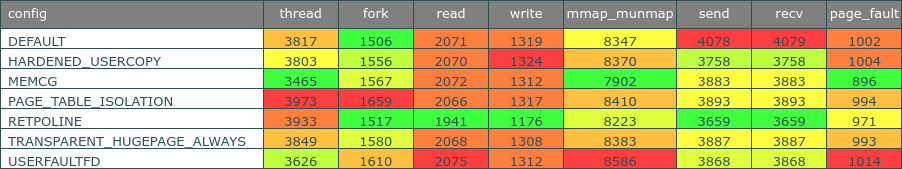
\includegraphics[width=\linewidth]{images/neon.png}
    \caption{AMD Ryzen 7 1700 @ 3.6 GHz}
\end{figure}

\begin{figure}[H]
    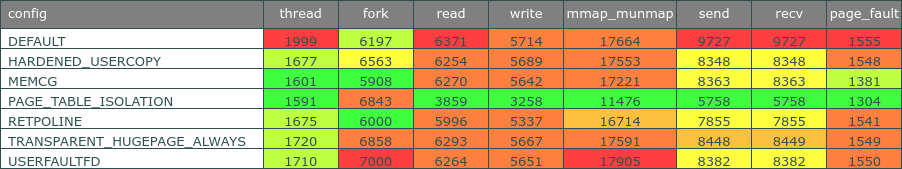
\includegraphics[width=\linewidth]{images/jelena.png}
    \caption{Intel Core i7--6500U @ 2.5 GHz}
\end{figure}

\begin{figure}[H]
    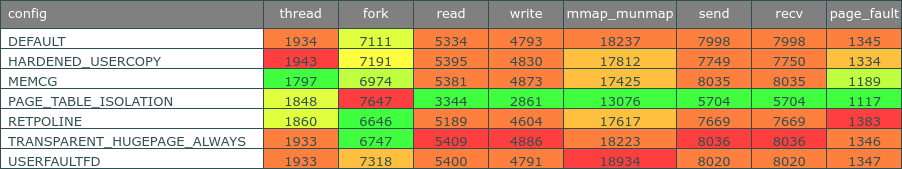
\includegraphics[width=\linewidth]{images/natrium.png}
    \caption{Intel Core i5--3320M @ 2.6 GHz}
\end{figure}

Iz priloženog se primećuje da različite konfiguracije Linux jezgra znatno utiču na vreme izvršavanja pojedinih sistemskih poziva. Pošto je uzrok promene u vremenu paljenje i gašenje pojedinih funkcionalnosti jezgra, nije potrebno ispitivanje razloga koji dovodi do promene performansi.

\subsection{Nalaženje najboljeg načina za poboljšanje performansi sistema}
Računari u današnje vreme imaju široki spektar primene i samim tim su im potrebna različite konfiguracije parametara jezgra. Neka podešavanja je moguće izmeniti, dok su druga neophodna za određene primene. Samim tim ne postoji savršeno rešenje za pitanje izbora parametara. Uloga svakog od testiranih konfiguracionih parametara je objašnjena u četvrtom poglavlju.

\section{Integracija}
Pošto ovo merenje performansi nije takmičarsko merenje i ne služi za kreiranje komercijalnog proizvoda, integracija se znatno olakšava. Potrebno je podesiti konfiguracione parametre Linux jezgra, prevesti ga i instalirati na računaru.

\chapter{Arhitektura}
\section{Linux jezgro}
Linux jezgro operativnog sistema je softver otvorenog koda, što znači da svaki korisnik može da preuzme celokupan kod sa interneta i prevede ga za lični računar. Pored toga što se neke funkcionalnosti Linux jezgra mogu kontrolisati tokom vremena izvršavanja, nudi i mnoštvo konfiguracionih parametara tokom prevođenja. Ti parametri ne utiču samo na mogućnosti jezgra, već mogu menjati i način rada internih komponenti (modula). Shodno tome, menjaju se i performanse jezgra, tj vreme izvršavanja koda tih modula.

Cilj rada je da utvrdi koje konfiguracije imaju najveći uticaj na performanse na razne sistemske pozive. Lista parametara nad kojima je izvršeno testiranje je preuzeta iz istraživačkog rada koji je ispitivao performanse različitih verzija jezgra~\cite{paper}.

Ostatak ove sekcije objašnjava svaki parametar, njegov uticaj na jezgro, kao i očekivani uticaj na performanse.

\subsection{CONFIG\_HARDENED\_USERCOPY}
\textit{Hardened usercopy} dodaje dodatne (i ponekad redundante) provere validnosti kernel pokazivača prilikom kopiranja podataka iz prostora jezgra u korisnički prostor i obrnuto. Te provere mogu imati nezanemarljiv uticaj na trajanje operacije kopiranja.

\subsection{CONFIG\_MEMCG}
\textit{CGroup memory controller}, memorijski kontroler za kontrolne grupe zabeležava i ograničava zauzeće memorije različitih kontrolnih grupa (\textit{cgroups}). Dozvoljava granularnu kontrolu nad resursima i jedna je od glavnih gradivnih jedinica za tehnologije kontejnerizacije procesa kao što su Docker i LXC\@. Ovaj modul može imati značajan uticaj na procese koji intenzivno koriste kontroler memorije jezgra, iako ne koriste mogućnosti kontrolera memorije kontrolnih grupa.

\subsection{CONFIG\_PAGE\_TABLE\_ISOLATION}
Izolacija jezgarne tabele stranica od korisničkog prostora je dodata kao sigurnosna zakrpa za izbegavanje \textit{Meltdown} ranjivosti prisutna kod velikog broja procesora. Uticaj na performanse varira od procesora i programa koji se izvršava, ali sa obzirom da eksploatisanje ranjivosti zahteva pokretanje malicioznog programa, ovaj parametar se može ugasiti za sisteme na kojima je garantovano da se pokreće isključivo provereni kod, kao na primer\ HPC proračuni.

\subsection{CONFIG\_RETPOLINE}
Izbegavanje spekulacije indirektnih grana je mera zaštite od \textit{Spectre V2} ranjivosti prisutna u modernim procesorima. Ovaj parametar kontroliše prisutnost zakrpe za izbegavanje te ranjivosti u kodu jezgra. Indirektna grana je skok u programskom kodu čiji cilj se ne može utvrditi statički, već samo tokom vremena izvršavanja. Moderni Intel i AMD procesori predviđaju koja će se grana najverovatnije izvršiti i nastavljaju sa izvršavanjem kako se ne bi prekinuo tok instrukcija. Problem je u tome što procesori ne eliminišu sve sporedne efekte prilikom pogrešne predikcije, npr.\ tako što ostave podatke u keš memoriji, što dovodi do toga da pažljivo izvršen maliciozan program može izvući poverljive podatke direktno iz procesora. Zakrpa je da se svako mesto u kodu jezgra, gde može doći do pogrešne predikcije, popuni takozvanim \textit{thunk} segmentom, koji se u suštini sastoji od beskonačne petlje.

\subsection{CONFIG\_TRANSPARENT\_HUGEPAGE\_ALWAYS}
Podrazumevane velike stranice dozvoljavaju jezgru da uvek odvoji veliku stranicu (2M) umesto osnovne (4K), što dovodi do smanjena tabele stranica i smanjuje broj \textit{pagefault} grešaka. Sa druge strane, može imati i negativan uticaj na performanse. Može dovesti do interne fragmentacije unutar stranica. Postoji i pozadinska nit koja povremeno osnovne stranice unapredi u velike, ali i troši procesorsko vreme. Razlika u performansi zavisi od načina korišćenja memorije, pa je teško meriti performanse za ovaj parametar.

\subsection{CONFIG\_USERFAULTFD}
Rukovanje \textit{pagefault} greškom u korisničkom prostoru ima primena za virtuelne mašine, ali sa sobom nosi i smanjenje performansi nekih sistemskih poziva, najiviše za \texttt{fork}. Razlog je što, prilikom kreiranja procesa, sistemski poziv mora proveriti za svaku memorijsku regiju roditelja da li ima informacije o rukovanju \textit{pagefault} greškama u korisničkom prostoru i preneti informaciju na regiju u procesu deteta.

\section{Distribucija}
Izvorni kod Linux jezgra je javno dostupan i proces prevođenja u binarnu datoteku je prost i jasno dokumentovan. Ono što nedostaje su korisničke aplikacije i ostatak operativnog sistema. Kad je u pitanju Linux jezgro, postoji mnoštvo takozvanih distribucija, koje nude celokupan operativni sistem sa korisničkim aplikacijama i svim što je potrebno da bi sistem bio funkcionalan.

Distribucija koja je izabrana za ovo testiranje je Arch Linux. Glavne prednosti ove distribucije su prilagodljivost i minimalnost. Minimalna instalacija troši veoma malo resursa pošto nema grafički interfejs i pozadinske servise koji nisu potrebni za osnovni rad operativnog sistema.

Pored toga, nudi i alate za kreiranje prilagođenih paketa (\textit{eng.\ package}), uključujući i samog jezgra. Za merenje performansi sistemskih poziva, kreirane su datoteke sa konfiguracijama za prevođenje jezgra sa izmenjenim parametrima koji su navedeni u prethodnoj sekciji, a zatim pokrenuta skripta koja prevodi kod jezgra i pakuje u izlaznu datoteku (paket).

Podrazumevana konfiguracija jezgra na Arch Linux distribuciji je prilagođena da obuhvata veliki broj računara. Zbog toga se proces prevođenja i pakovanja izvršava samo jednom na jednom računaru, pa se zatim izlazne datoteke prenose na ostale kako bi se štedelo na vremenu i garantovalo da će jezgra biti identična na svim računarima.

Git repozitorijumu sa svim konfiguracijama i skriptama za pokretanje je javno dostupan~\cite{repo:runner}

\chapter{Sistemski pozivi}
Sistemski pozivi su način na koji korisnički programi zahtevaju razne operacije od jezgra operativnog sistema. To uključuje operacije za komunikaciju sa eksternim uređajima (npr.\ pristup disku), kreiranje i izvršavanje novih procesa, zauzimanje i oslobađanje memorije, itd. Sistemski pozivi čine neophodan interfejs između procesa i operativnog sistema.

U ovom projektu, sistemski pozivi su pozivani pomoću programskog jezika \textit{C} i odgovarajućih biblioteka za neke od poziva, što je prikazano u nastavku teksta. Svaki sistemski poziv se testira u okviru različitog programa, a za pokretanje tih programa i prikazivanje rezultata zadužena je \textit{Bash} skripta.

Za merenje vremena koje je potrebno za izvršavanje sistemskih poziva koristi se biblioteka \texttt{sys/time.h} koja zabeleži sistemsko vreme pre pozivanja sistemskog poziva:
\begin{minted}{c}
    struct timeval start;
    gettimeofday(&start, NULL);
\end{minted}
i nakon izvršenja sistemskog poziva:
\begin{minted}{c}
    struct timeval stop;
    gettimeofday(&stop, NULL);
\end{minted}

Oduzimanjem ova dva trenutka, dobija se vreme koje je bilo potrebno za izvršavanje koda koji se nalazi između ovih naredbi.

Kod za pozivanje svakog sistemskog poziva je javno dostupa na Git repozitorijumu~\cite{repo:syscalls}

\section{Fork}
\textit{Fork} sistemski poziv služi za kreiranje novog procesa sa identičnim kontekstom kao trenutni. Program kao argument komandne linije prima broj $ n $ koji označava broj poziva sistemskog poziva fork. Nakon $ n $ poziva, postojaće $ 2^n $ procesa. Poziv sistemskog poziva izgleda ovako:
\begin{minted}{c}
    syscall(SYS_fork);
\end{minted}

Povratna vrednost poziva fork je id procesa deteta u roditeljskom procesu, odnosno 0 u novonastalom procesu. Izmereno vreme je vreme koje se izmeri nakon kreiranja poslednjeg procesa.

\section{Read}
\textit{Read} sistemski poziv služi za čitanje sadržaja datoteka iz sistema datoteka. Program kao argument komandne linije prima broj koji označava broj izvršavanja sistemskog poziva read. Svaki poziv izgleda ovako:
\begin{minted}{c}
    syscall(SYS_read, fileno(f), &c, n);
\end{minted}
gde je \texttt{fileno(f)} deskriptor fajla iz kojeg se čita, \texttt{c} promenljiva u koju se smešta pročitani sadržaj i \texttt{n} broj bajtova koji se čitaju.

Povratna vrednost sistemskog poziva read je broj pročitanih bajtova ako je čitanje uspešo, 0 ako se dođe do kraja fajla ili -1 ako čitanje nije uspešno.

\section{Write}
\textit{Write} sistemski poziv služi za upisivanje sadržaja u datoteke. Program kao argument komandne linije prima broj koji označava broj izvršavanja sistemskog poziva write. Svaki poziv izgleda ovako:
\begin{minted}{c}
    syscall(SYS_write, fileno(f), text, n);
\end{minted}
gde je \texttt{fileno(f)} deskriptor fajla u koji se piše, \texttt{text} sadržaj koji se piše u fajl i \texttt{n} broj bajtova koji se upisuju u fajl.

Povratna vrednost sistemskog poziva write je broj upisanih bajtova ako je pisanje uspešo ili -1 ako pisanje nije uspešno.

\section{Mmap i munmap}
\textit{Mmap} povezuje adresni prostor procesa sa objektom u RAM memoriji. \textit{Munmap} sistemski poziv je zadužen da ukloni vezu koju \textit{mmap} kreira. Pošto su operacije usko povezane, njihovo vreme izvršavanja se meri zajedno. Program kao argument komandne linije prima broj izvršavanja sistemskih poziva \textit{mmap} i \textit{munmap}, $ n $ i broj memorijskih stranica koje se mapiraju, \texttt{pages}. Svaki od $ n $ poziva prvo izvršava \textit{mmap}, pa nakon njega \textit{munmap} sistemski poziv.

\begin{samepage}
    \textit{mmap}:
    \begin{minted}{c}
            char* region = mmap(
                (void*) pagesize,
                pages* pagesize,
                PROT_READ|PROT_WRITE|PROT_EXEC,
                MAP_ANON|MAP_PRIVATE,
                0,
                0
            );
    \end{minted}
\end{samepage}

\textit{munmap}:
\begin{minted}{c}
        munmap(region, pages * pagesize);
\end{minted}

\textit{Mmap} kao parametre prima \texttt{(void*) pagesize} kao početnu adresu regiona koji se mapira, \texttt{pages * pagesize} kao veličinu adresnog prostora koji se mapira, \texttt{PROT\_READ|PROT\_WRITE|PROT\_EXEC} kao permisije, \texttt{MAP\_ANON|MAP\_PRIVATE} kao \texttt{flags} parametar koji dodatno opisuje način mapiranja i naredna dva parametra koja očekuju deskriptor fajla i pomeraj u odnosu na početak fajla. Povratna vrednost ovog sistemskog poziva je pokazivač na početak mapiranog bloka.

\textit{Munmap} kao parametre prima \texttt{region} kao početnu adresu regiona i \texttt{pages* pagesize} kao veličinu adresnog prostora čije mapiranje se uklanja. Povratna vrednost ovog sistemskog poziva je 0 ako se uspešno izvrši, odnosno -1 ako se neuspešno izvrši.

\texttt{Pagesize} je veličina jedne memorijske stranice.

\section{Page fault}
\textit{Page fault} nije eksplicitan sistemski poziv, već je izuzetak koji se desi kada pokrenuti program pristupa memorijskoj stranici koja nije trenutno mapirana u virtuelni adresni prostor procesora. Nakon ovog događaja, sistem za upravljanje izuzetcima pokuša da dobavi traženu stranicu i da je mapira. Program kao argument komandne linije prima broj izazivanja page fault izuzetka. Jedno izazivanje page fault izuzetka izgleda ovako:

\begin{minted}{c}
    unsigned char *p = malloc(pagesize + 1);
    p[0] = 0;
\end{minted}

Velika je verovatnoća da se pri pozivu \texttt{p[0] = 0;} stranica koja je potrebna ne nalazi u memoriji i time će se pokrenuti obrada page fault izuzetka.

\texttt{Pagesize} je veličina jedne memorijske stranice.

\section{Send i recv}
\textit{Send} sistemski poziv je zadužen da pošalje poruku drugom soketu. \textit{Recv} je zadužen da primi poruku iz soketa. Za merenje vremena izvršavanja ova dva poziva, koristi se klijent-server aplikacija gde klijent šalje poruke pomoću \textit{send}-a, a server prima poruke pomoću \textit{recv}-a.

Serverska aplikacija nakon pokretanja očekuje konekciju sa klijentskom aplikacijom. Nakon konekcije, serverska aplikacija kreće da meri vreme i osluškuje poruke koje stižu sa klijentske aplikacije. Kada stigne poruka \texttt{exit}, osluškivanje poruka i merenje vremena se obustavljaju. \textit{Recv} sistemski poziv u serverskoj aplikaciji prikazan je u narednom kodu:

\begin{minted}{c}
    recv(sockfd, buff, sizeof(buff), 0);
\end{minted}
gde \texttt{sockfd} predstavlja fajl deskriptor soketa koji šalje poruku, \texttt{buff} i \texttt{sizeof(buff)} predstavljaju promenjivu u koju se smešta primljeni tekst i njenu dužinu i, kao poslednji parametar, \texttt{flags} ova funkcija može da primi dodatna podešavanja za primanje poruka.

Povratna vrednost sistemskog poziva \textit{recv} je broj primljenih bajtova ako je primanje uspešo ili -1 ako primanje nije uspešno.

Klijentska aplikacija kao argument komandne linije prima broj poruka, $ n $ i tekst koji će poslati, konektuje se na serversku aplikaciju i zatim vrši slanje poruka:

\begin{minted}{c}
    send(sockfd, buff, sizeof(buff), 0);
\end{minted}

Parametri ovog sistemskog poziva imaju isto značenje kao i parametri kod primanja poruka, samo u kontekstu slanja poruka.

Povratna vrednost sistemskog poziva \textit{send} je broj poslatih bajtova ako je slanje uspešo ili -1 ako slanje nije uspešno.

Nakon slanja svih poruka, šalje se poruka \texttt{exit} da naznači serverskoj aplikaciji da su poslate sve poruke. Kod klijentske aplikacije, vreme se meri od početka slanja poruka do slanja poslednje poruke.

\section{Thread}
Ova sekcija je zadužena da prikaže način merenja vremena koje je potrebno za kreiranje i uništavanje niti. Program kao argument komandne linije prima broj koji označava broj niti koje se kreiraju. Za svaku od niti izvrši se sledeći kod:
\begin{minted}{c}
pthread_create(&thread_id, NULL, threadFun, NULL);
pthread_join(thread_id, NULL);
\end{minted}
i meri vreme koje je potrebno da se kod izvrši. Prva komanda kreira nit i identifikator niti sačuva u promenjivoj \texttt{thread\_id}. Nakon toga pozove funkciju \texttt{threadFun()} bez parametara. Druga komanda čeka da se izvrši funkcija \texttt{threadFun()} bez da sačuva povratnu vrednost i nakon toga uništi nit.

\chapter{Zaključak}
Iz izmerenih vremena izvršavanja u~\hyperref[benchmark]{sekciji 3.2.2} se prvobitno vidi razlika između Intel i AMD sistema. Kod Intel sistema izolacija jezgarne tabele stranica ima značjano veći uticaj na performanse nego kod AMD sistema. Obrnuto od toga, gašenje \textit{Spectre} mitigacije, daje značajniji porast performansama na AMD sistemima.

Za ostale parametre se u većini slučajeva dobijaju bolje performanse ako su ugašeni (podrazumevano su upaljeni), sem kod nekih izuzetaka kao npr.\ \textit{fork} sistemski poziv uz \texttt{PAGE\_TABLE\_ISOLATION} parametar ugašen. Pretpostavka je da sa spojenim tabelama stranica, operativni sistem mora da prođe kroz više stranica i napravi njihove kopije prilikom kreiranja novog procesa.

Dalje ispitivanje bi moglo da se radi nad različitim kombinacijama parametara što zahteva znatno veće vreme prevođenja jezgra i pokretanja merenja vremena izvršavanja, pošto broj kombinacija raste eksponencijalno sa svakim parametrom.

\chapter{Literatura}
\sloppy
\printbibliography[heading=none]

\end{document}
